\chapter{实验研究}\label{sec:experiments}
\setcounter{secnumdepth}{3}

财富路径影响参考点，参考点改变CPT评价，而策略更新又会改变下一条财富路径。为了逐步看清这些关系，前四组实验从路径比较出发，依次考察有限样本梯度、连续在线跟踪和参考点机制的作用；后三组实验转向真实A股价格、投资者持股决策及持续推荐。可控环境便于区分各环节的影响，真实数据则呈现组合表现与行为解释上的结果。七组实验的关系见图~\ref{fig:evidence-map}。

\begin{figure}[H]
    \centering
    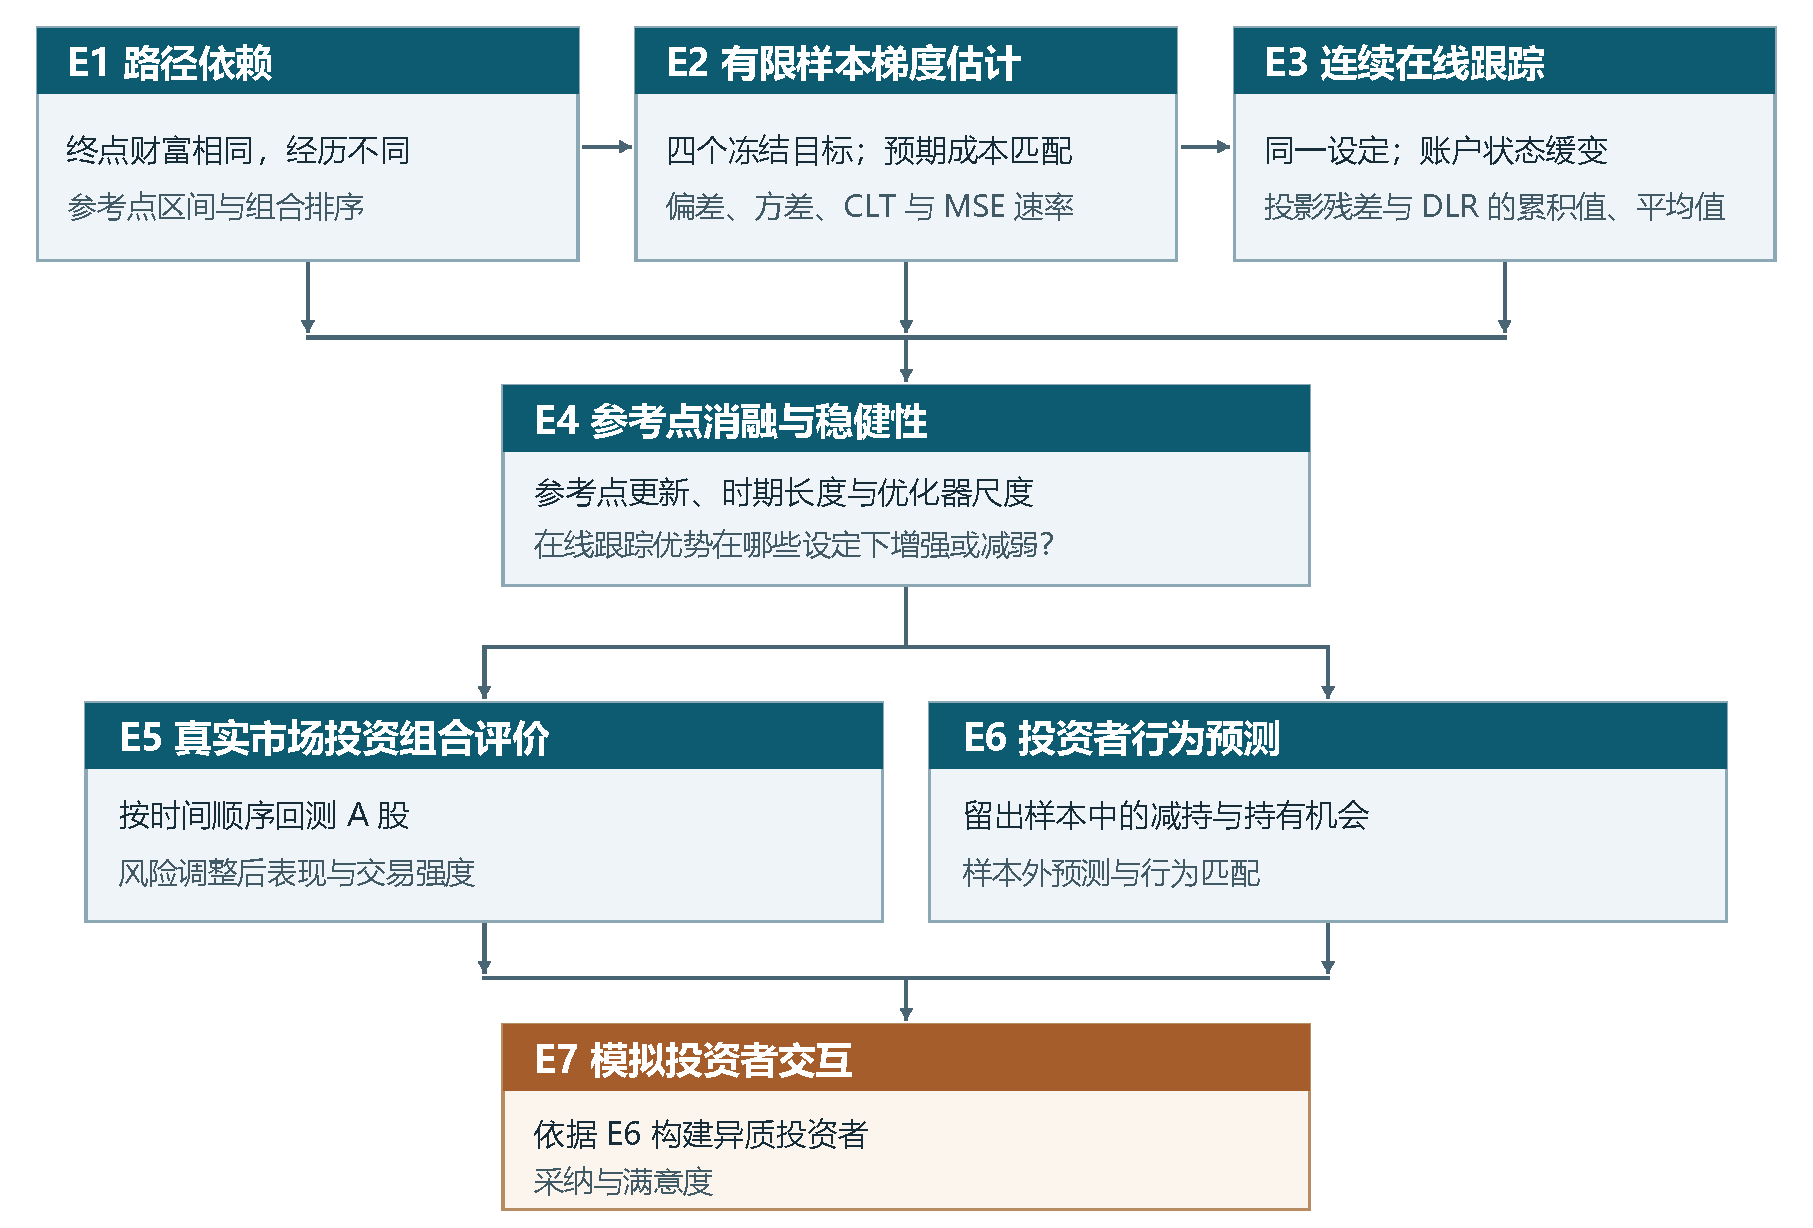
\includegraphics[width=0.96\textwidth]{figures/experiment_evidence_map_zh.pdf}
    \caption{七组实验之间的证据关系。}
    \label{fig:evidence-map}
\end{figure}

\section{E1：路径依赖与投资组合选择}\label{sec:e1}

为观察参考点如何把投资经历带入下一次选择，考虑两条初始财富和最终财富相同的路径：
\[
(1,1.10,1.015)\qquad\text{与}\qquad(1,0.90,1.015).
\]
参考点按式~\eqref{eq:reference-update}逐期更新，取$(\eta_+,\eta_-)=(0.20,0.05)$。到决策时，两位投资者的财富都为$X_T=1.015$，调仓前均持有$50\%$现金和$50\%$风险资产。下一期风险资产以概率$p$上涨$4\%$，否则下跌$4\%$。可选的目标风险权重为$20\%$和$80\%$；经过式~\eqref{eq:action-map}的动作惯性，实际执行权重分别为$44\%$和$56\%$。下一期只有两种收益状态，故两种配置的CPT价值均可精确计算。

图~\ref{fig:e1-path-choice}A先画出两条财富路径及参考点的变化，B对照动态、对称动态和静态参考点下的期末盈亏位置；C、D则分别沿两条路径改变上涨概率，比较两种可执行配置的CPT价值。

\begin{figure}[!htbp]
    \centering
    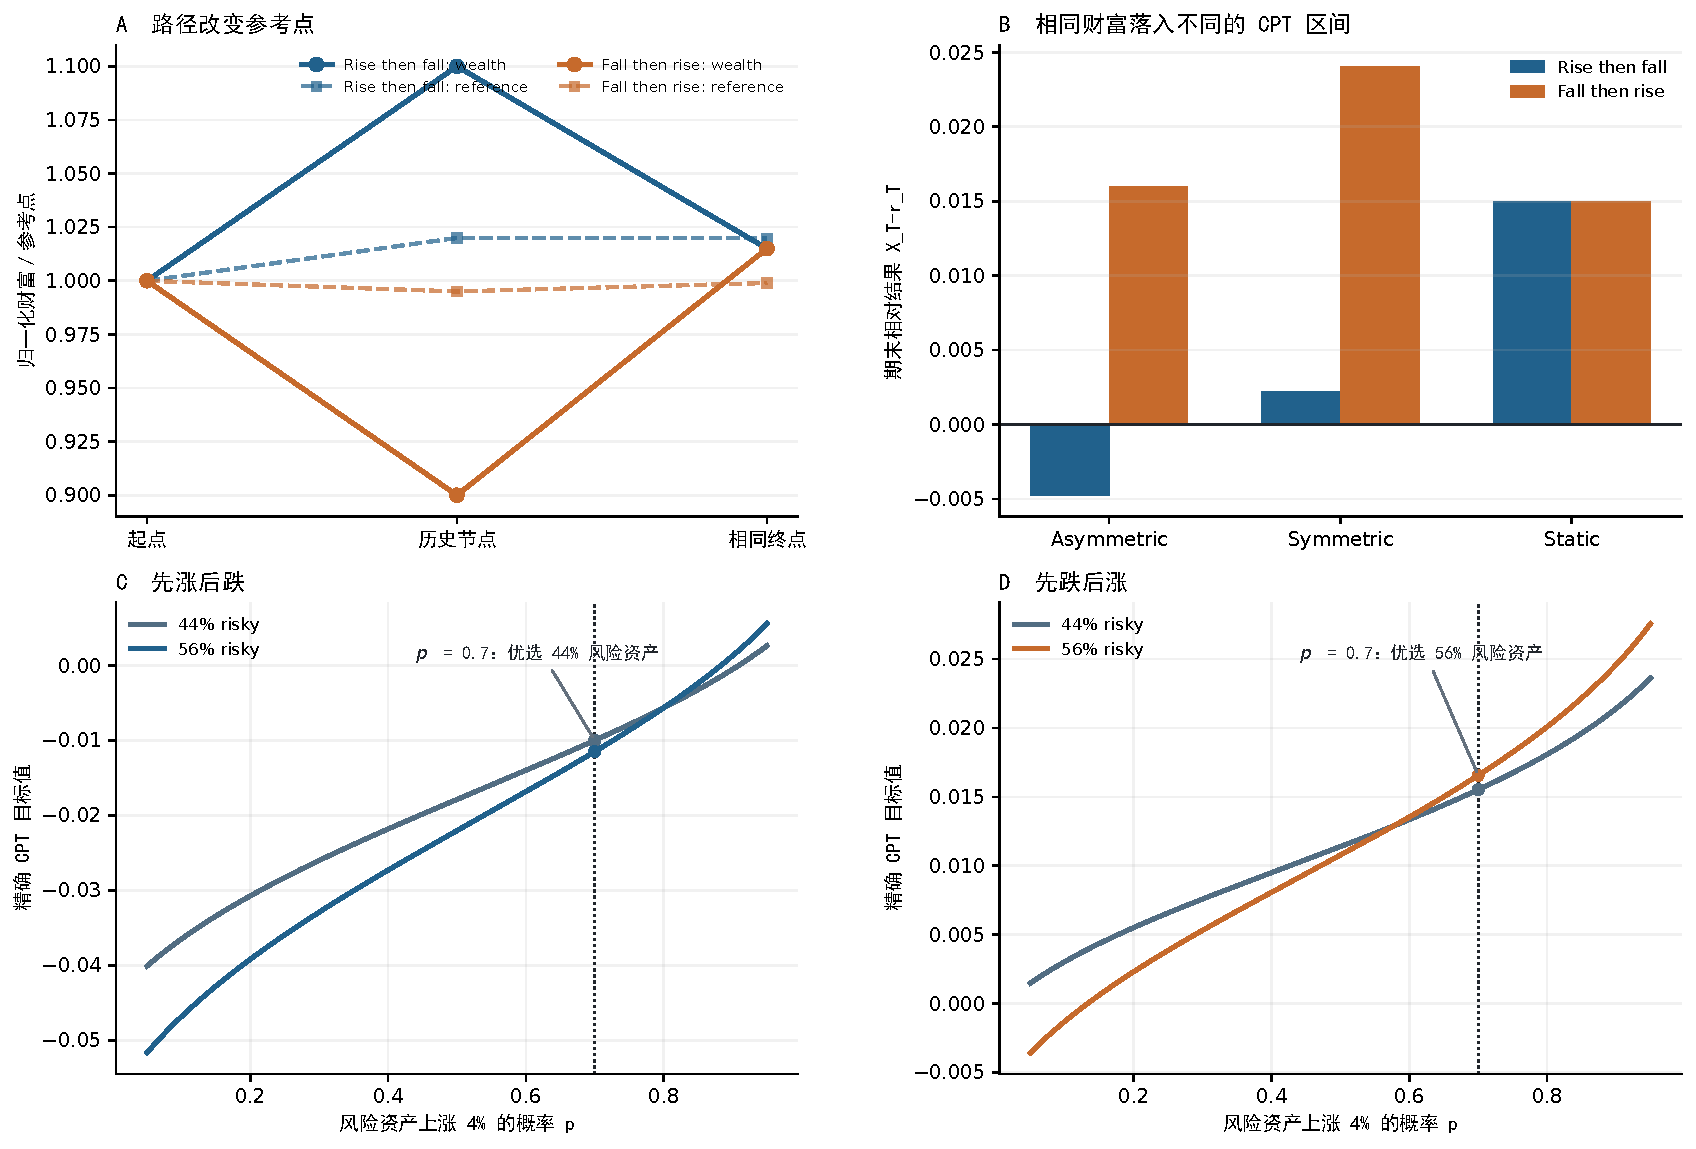
\includegraphics[width=\textwidth]{figures/e1_path_and_decision_final_zh.pdf}
    \caption{财富路径、参考点与投资组合选择}
    \label{fig:e1-path-choice}
\end{figure}

\begin{table}[!htbp]
\centering
\caption{E1在$p=0.7$时的精确机制结果。}
\label{tab:e1-summary}
\setlength{\tabcolsep}{4.8pt}
\begin{tabular}{lrrrrl}
\toprule
财富路径 & $X_T$ & $r_T$ & $X_T-r_T$ & 优选风险资产权重 & CPT区间 \\
\midrule
先涨后跌 & 1.015 & 1.01975 & $-0.00475$ & 44\% & 损失 \\
先跌后涨 & 1.015 & 0.99900 & $+0.01600$ & 56\% & 收益 \\
\bottomrule
\end{tabular}
\end{table}

两条路径最终都到达$1.015$，但先涨后跌的账户留下较高参考点，$X_T-r_T=-0.00475$；先跌后涨的账户则处于参考点之上，$X_T-r_T=0.016$。因此，面对相同的$\{+4\%,-4\%\}$下一期收益，前者主要从损失一侧评价风险，后者则从收益一侧评价。上涨概率取$p=0.7$时，前者选择$44\%$风险资产，后者选择$56\%$（图~\ref{fig:e1-path-choice}）。财富、持仓和可选配置均已配平，排序的反转来自历史路径留下的参考点差异，与命题~\ref{prop:path-dependence}所揭示的机制一致。

\FloatBarrier
\section{E2：有限样本梯度估计}\label{sec:e2}

单凭真实价格路径，难以知道梯度估计误差究竟来自方法本身，还是来自不断变化的市场。从E2开始，实验采用$30$只股票加现金的半合成市场：各股因子来自固定的A股经验因子块库，收益规律则按预设路径变化。股票之间仍有真实因子差异，而市场何时突变、何时缓变可以明确控制。时期$k$内，风险资产$i$在第$u$日的收益为
\[
R_{i,k,u}=0.08\,\tanh\!\left(
\frac{\mu_k^{\rm ret}+2.5\,(\phi_k^{\rm ret})^\top f_{i,u}+\xi^{\rm com}_{k,u}+\xi^{\rm id}_{i,k,u}}{0.08}
\right),
\]
其中$f_{i,u}$是资产$i$的因子向量，$\phi_k^{\rm ret}$与其维度相同；共同冲击和个股冲击的标准差分别为$0.006\sigma_k^{\rm ret}$与$0.009\sigma_k^{\rm ret}$，$(\mu_k^{\rm ret},\phi_k^{\rm ret},\sigma_k^{\rm ret})$控制当期的收益规律。市场先在第$1$--$40$期保持动量规律，第$41$--$60$期转向反转，第$61$--$120$期逐渐过渡到低波动、价值和质量占优的状态；此后外生收益规律不再改变。这样，四个取样时期分别落在稳定、突变后、缓变中和缓变后的市场状态。

E2把账户条件统一为
\[
(X,r,\omega,\theta)=(1,1,e_{\rm cash},0),
\qquad e_{\rm cash}:=(1,0,\ldots,0),
\]
并在第$20$、$50$、$90$和$150$期分别冻结一个目标，对应稳定、突变后、缓变中和缓变后的市场状态。E3沿用同一因子分布和时期收益规律，但让账户状态在各期之间连续演化。

我们比较本文采用的中心化留一估计器（带独立原始随机修正）与改编自CPT-PG v5的原始独立分割plug-in估计器。两者估计的都是式~\eqref{eq:value-functions}中的平方平滑CPT目标。预期完整轨迹预算取
\[
\mathsf B\in\{32,64,128,256,512,1024,2048\},
\]
两种方法在每一预算下匹配轨迹成本，数值梯度参照值由独立且成本高得多的模拟产生。

图~\ref{fig:e2-estimator}A比较固定目标上的坐标偏差，B考察独立估计量取平均后的协方差迹，C在$M=64$时检查标准化统计量的正态分位数，D比较不同因子维度下全梯度MSE随预算的变化。B、D中的虚线均表示斜率为$-1$的参照线。

\begin{figure}[!htbp]
    \centering
    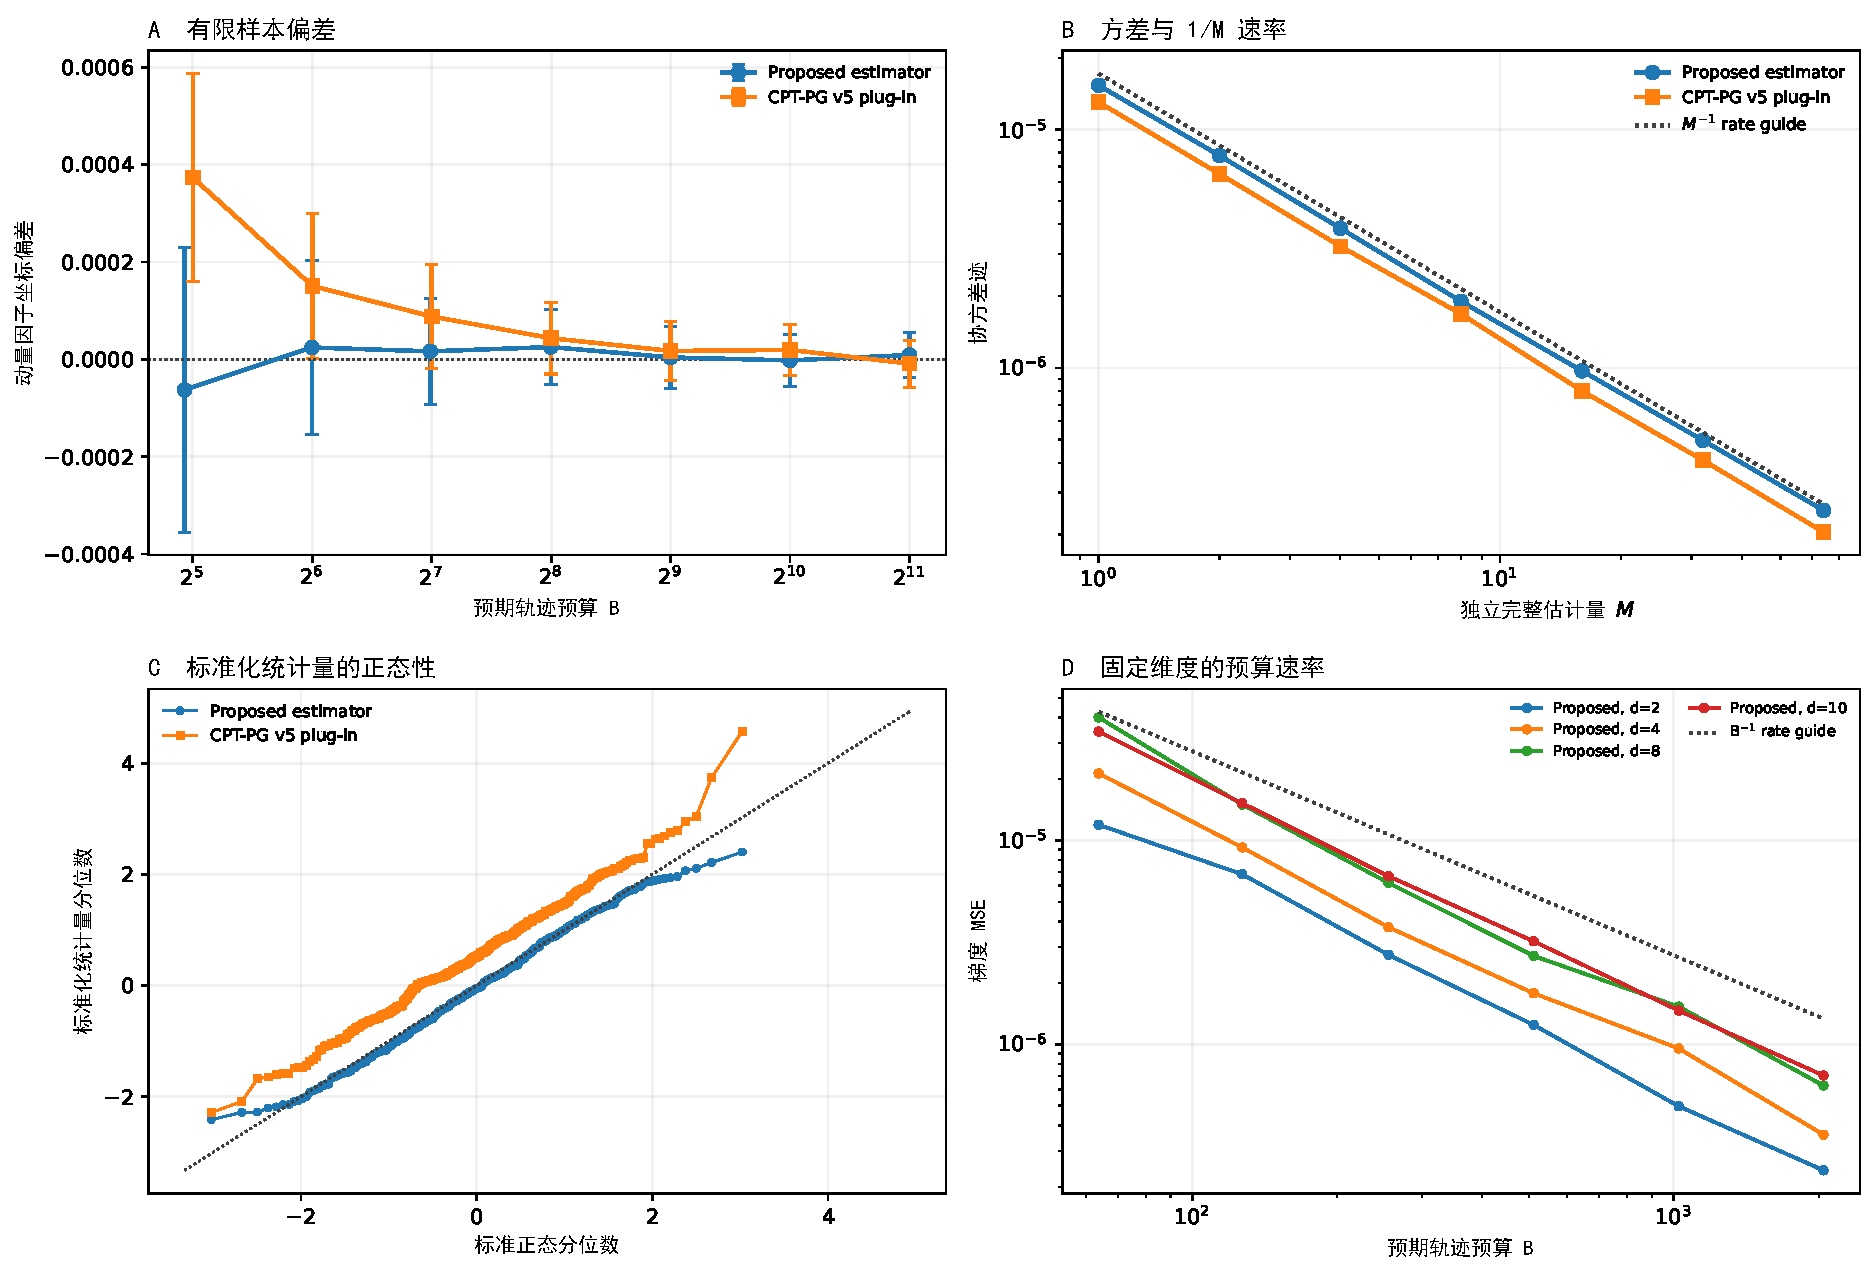
\includegraphics[width=\textwidth]{figures/e2_estimator_diagnostics_zh.pdf}
    \caption{半合成环境中的有限样本梯度估计}
    \label{fig:e2-estimator}
\end{figure}

\begin{table}[!htbp]
\centering
\small
\caption{四个固定目标在预期轨迹预算$\mathsf B=512$时的全梯度均方误差。MSE数值单位为$10^{-6}$；末列为$\mathrm{MSE}_{\rm prop}-\mathrm{MSE}_{\rm v5}$的配对$95\%$ bootstrap区间，单位相同。}
\label{tab:e2-period-mse}
\begin{tabular}{lrrrr}
\toprule
市场状态 & 本文估计器 & CPT-PG v5 & 比值 & 差值的95\% CI \\
\midrule
稳定期 & 3.123 & 2.938 & 1.063 & $[-0.055,\ 0.434]$ \\
突变后 & 10.134 & 10.809 & 0.938 & $[-1.495,\ 0.139]$ \\
缓变中 & 10.647 & 11.468 & 0.928 & $[-1.739,\ 0.102]$ \\
缓变后 & 10.589 & 12.257 & 0.864 & $[-2.599,-0.721]$ \\
\bottomrule
\end{tabular}
\end{table}

有限预算下，两种估计器首先在偏差上拉开距离。本文估计量的各坐标均值靠近独立数值参照值，CPT-PG v5的plug-in估计量在低预算时则出现偏移（图~\ref{fig:e2-estimator}A）。原因在于plug-in方法把经验生存概率直接送入非线性权重导数；留一中心化和独立随机修正则使这一有限样本偏移在期望上得到消除。

无偏并不意味着只用少量轨迹就能得到精确方向，因而还须看预算增加后的波动。独立完整估计量取平均时，两种方法协方差迹的拟合斜率分别为$-0.989$和$-0.999$；本文方法在$d=2,4,8,10$时，全梯度MSE的预算斜率介于$-1.17$与$-1.12$之间（图~\ref{fig:e2-estimator}B、D），与定理~\ref{thm:minimax}的逆预算率相吻合。固定$M=64$时，本文方法的标准化统计量均值为$-0.049$、标准差为$0.993$，$95\%$区间覆盖率为$96.25\%$；CPT-PG v5的均值为$0.556$，覆盖率为$91.75\%$（图~\ref{fig:e2-estimator}C）。前一组数字说明估计波动如何随预算下降，后一组数字则反映有限样本偏移对区间推断的影响。

MSE比较还取决于所处的市场状态。预算$\mathsf B=512$时，四个目标中有三个的MSE点估计较低；缓变结束后的降幅为$13.6\%$，配对区间全部在零以下，稳定期的点估计却略高且区间跨过零（表~\ref{tab:e2-period-mse}）。四个目标共同支持的是有限样本偏移得到修正、误差随预算增大以约$1/\mathsf B$的速度下降；在某一固定预算下，哪种方法的MSE更低还取决于目标状态。

\FloatBarrier
\section{E3：连续缓变环境中的在线跟踪}\label{sec:e3}

固定目标上的梯度估计只是策略更新的第一步。市场从动量转向反转、再逐渐改变因子偏好时，在线策略还需要沿着自己的账户路径继续运行。记第$k$期结束、跨期缓变处理之前的原始账户状态为$(X_k^{\rm raw},r_k^{\rm raw},\omega_k^{\rm raw})$。下一期从以下状态出发：
\[
\begin{aligned}
\log X_{t_{k+1}}
&=(1-\varpi_k)\log X_{t_k}+\varpi_k\log X_k^{\rm raw},\\
r_{k+1}
&=(1-\varpi_k)r_k+\varpi_k r_k^{\rm raw},\\
\omega_{t_{k+1}-1}
&=(1-\varpi_k)\omega_{t_k-1}+\varpi_k\omega_k^{\rm raw},
\qquad \varpi_k=k^{-3/4}.
\end{aligned}
\]
期内参考点仍按式~\eqref{eq:reference-update}非对称更新，$(\eta_+,\eta_-)=(0.20,0.05)$。在假设~\ref{ass:trajectory}的共同有界域和有界半合成收益下，期初状态变化量为$O(\varpi_k)$，且
\[
\sum_{k\le K}\varpi_k=O(K^{1/4})=o(K).
\]
因子块分布保持不变，外生收益系数沿E2的阶段路径变化至第$120$期，此后固定。跨期混合使账户承接上一期的经历，同时使后期状态每次移动的幅度逐渐缩小；期内的每日财富和参考点仍由实际交易路径决定。若冻结目标在所考察紧域内对期初账户变量和收益系数一致Lipschitz连续，附录~\ref{app:online}中的推导把这种状态变化转为$\cV_K=O(K^{1/4})$的目标变化预算。

实验使用$20$条独立测试轨迹。在线学习者与冻结对照在前$40$期共享完整路径；此后前者继续运行算法~\ref{alg:drcptpg}，后者固定$\theta$，但仍按相同缓变规则推进各自的财富、参考点和持仓。测试前设定$(\gamma,\vartheta)=(0.08,0.05)$，每期估计量独立重复$M_k=\max\{4,\lceil\sqrt{k}\rceil\}$次。因此$M_k\ge\sqrt{k}$，且$K^{-1}\sum_{k=1}^{K}M_k^{-1}\le(2\sqrt K-1)/K=O(K^{-1/2})$。动态局部遗憾按式~\eqref{eq:dynamic-regret}计算，取$W=5$、$\rho=0.9$。为避免将评估梯度的抽样波动直接计入平方残差，图中使用两条独立梯度流的交叉乘积，分别评价当期投影残差和经式~\eqref{eq:dynamic-window-residual}平滑后的残差；相应误差界见式~\eqref{eq:cross-stream-residual-error}和\eqref{eq:cross-stream-dlr-error}。

图~\ref{fig:e3-tracking}A、B依次给出平方投影残差的累计值和时期平均值，C、D以同样方式给出动态局部遗憾。竖直点线标出市场突变、缓变开始及外生收益规律固定的时点；曲线是$20$条测试轨迹的均值，阴影为$1.96$倍标准误。

\begin{figure}[!htbp]
    \centering
    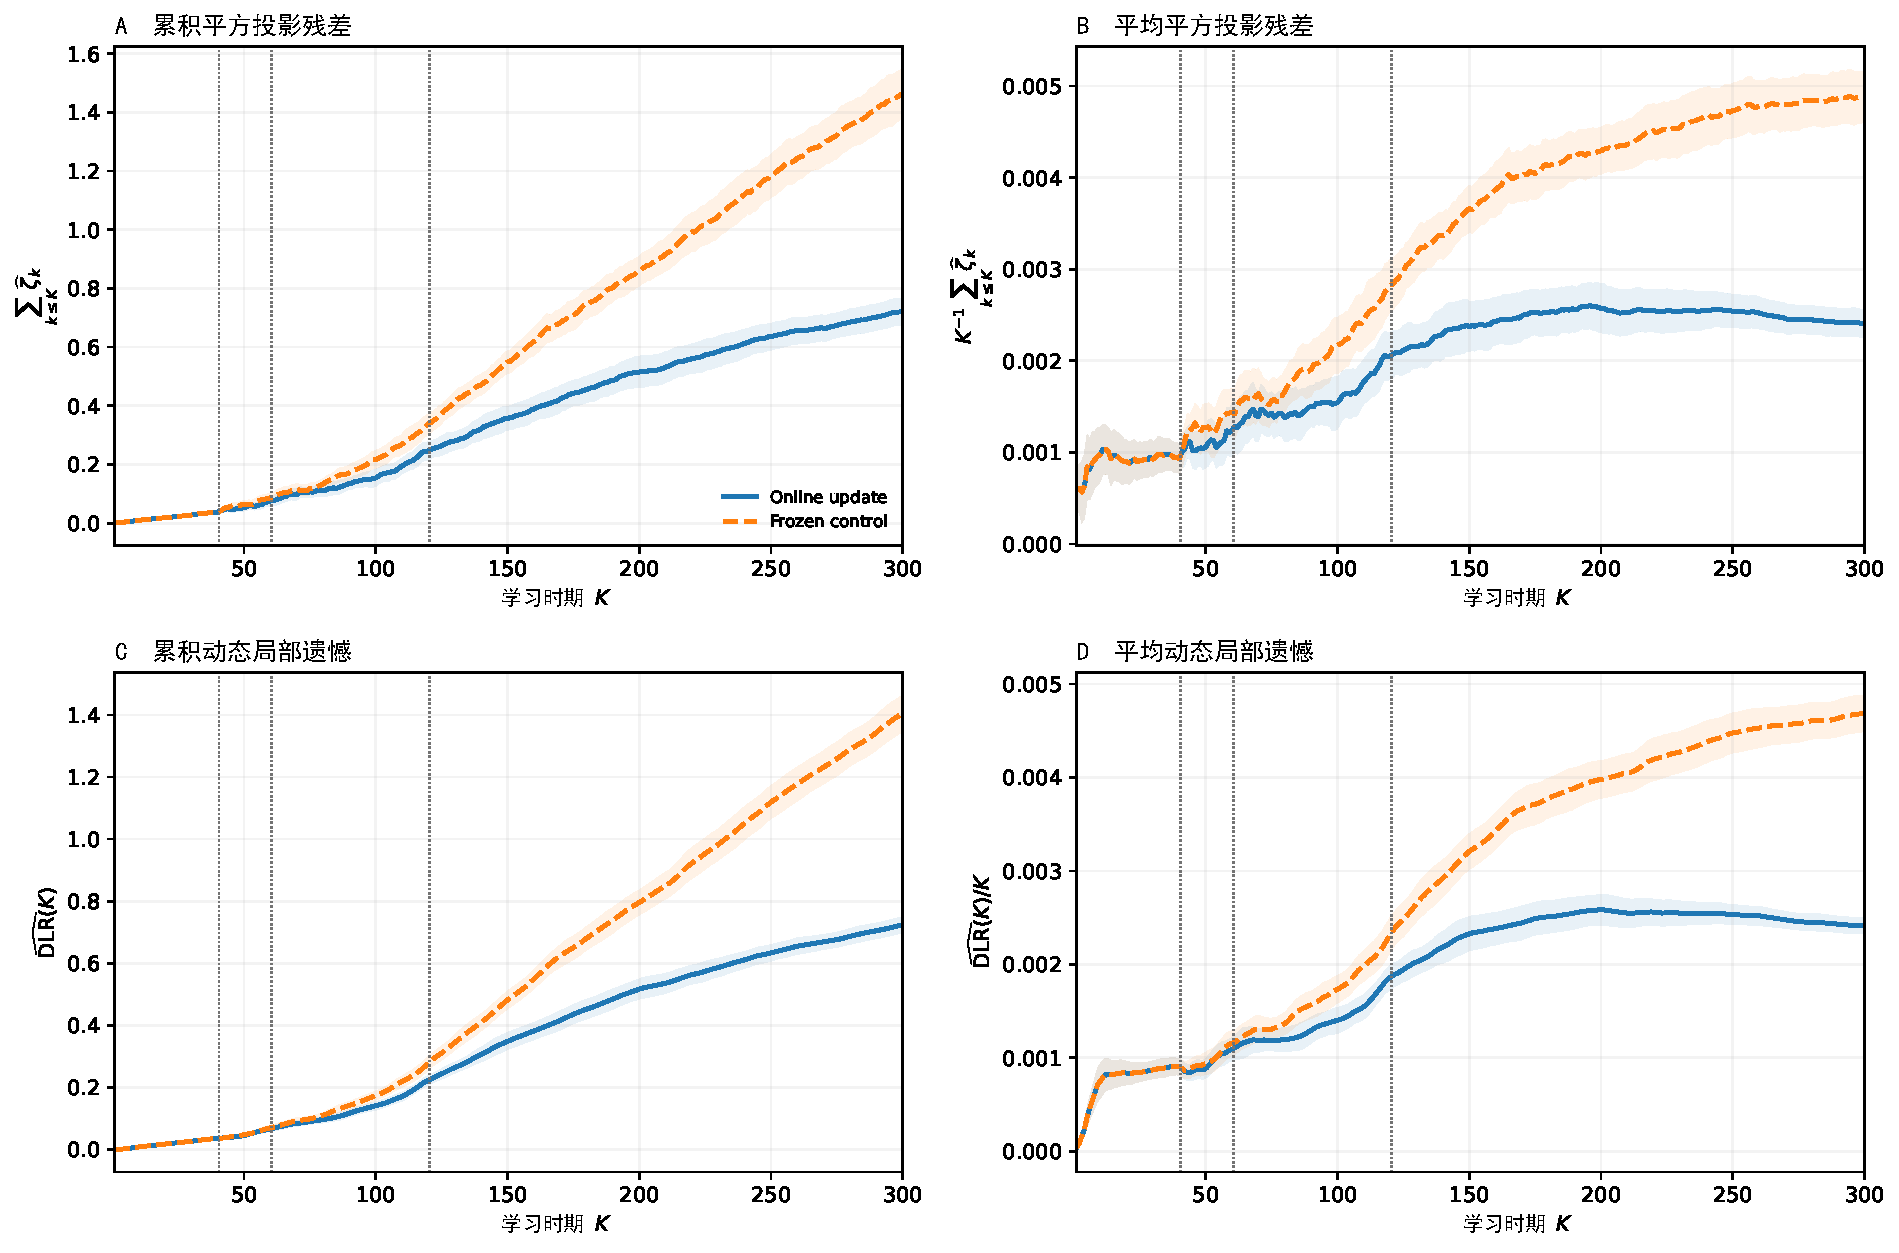
\includegraphics[width=\textwidth]{figures/e3_online_tracking_zh.pdf}
    \caption{缓变环境中的连续在线跟踪}
    \label{fig:e3-tracking}
\end{figure}

前$40$期，两组账户走过同一条路径；参数冻结后，持续更新组与对照组的残差逐渐分开（图~\ref{fig:e3-tracking}）。第$41$期至第$300$期，持续更新组的动态局部遗憾累计为$0.687$，约为冻结对照$1.369$的一半；直接累计平方投影残差也得到相近的差距（$0.684$对$1.427$）。两项差值按种子配对的$95\%$ bootstrap区间分别为$[-0.738,-0.622]$和$[-0.834,-0.650]$。到第$300$期，两组平均动态局部遗憾分别为$2.411\times10^{-3}$和$4.685\times10^{-3}$。冻结策略仍继续持仓、经历市场并更新参考点，因此差距反映的是持续修正参数能否更好地跟上各自当期的CPT目标。

第$121$期以后，外生收益规律已经固定，目标的继续移动主要来自缓变的账户状态。在第$121$--$300$期，累积动态局部遗憾的经验双对数斜率，持续更新为$0.704$，冻结对照为$0.968$；平方投影残差的斜率分别为$0.745$和$0.959$。持续更新曲线在这一有限区间内呈现低于线性的积累趋势，与推论~\ref{cor:dynamic-local-regret}和\ref{cor:vanishing-tracking}描述的渐近方向一致。在式~\eqref{eq:error-bound}的局部几何条件下，残差控制还能按推论~\ref{cor:stationary-tracking}转化为到当期驻点集合的平均平方距离控制。市场不再改变收益规律之后，账户仍记着此前的交易经历；持续修正参数因而仍比停留在第$40$期的策略更贴近当期目标。

\FloatBarrier
\section{E4：参考点机制消融与在线跟踪稳健性}\label{sec:e4}

持续更新在E3的默认配置下优于冻结策略，但这一差距可能随参考点适应速度、每期长度和参数更新尺度改变。参考点若保持不变，持续学习还是否有用？收益后与损失后采用不同的适应速度，又会把差距推向哪一边？为使不同配置的比较不受目标尺度影响，对配置$c$和配对种子$s$，计算突变后在线策略与冻结策略的动态局部遗憾比值
\[
\mathrm{Ratio}_{\mathrm{DLR}}(c,s)
=\frac{\mathrm{DLR}^{\rm post}_{\rm online}(c,s)}{\mathrm{DLR}^{\rm post}_{\rm frozen}(c,s)}.
\]
先在每个种子内求比值，再计算其平均值和配对bootstrap区间。比值小于一，表示该配置下持续更新比冻结参数积累更少的动态局部遗憾。

首先在完整的$9\times9$参考点网格中改变收益和损失后的适应速度：
\[
\eta_+,\eta_-\in\{0,0.05,0.10,\ldots,0.40\}.
\]
随后将时期长度设为
\[
h\in\{1,5,10,15,20,25,30,35,40,45,50\};
\]
市场阶段仍按第$200$、$300$、$600$、$1500$个交易日界定；当边界落在一个时期内部时，归入最近的完整时期，跨期状态增益则按已经经过的交易日计算。最后考察更新步长与归一化下界，从
\[
\gamma\in\{0.01,0.02,0.03,0.04,0.05,0.06,0.08,0.10,0.12\},
\]
\[
\vartheta\in\{0.005,0.01,0.015,0.02,0.03,0.04,0.05,0.06\},
\qquad 0.31\,\gamma\le\vartheta
\]
中筛出$48$组配置；这里的$0.31$为网格筛选系数。每组配置运行四条独立配对轨迹和两条独立评估流。

图~\ref{fig:e4-robustness}A是$9\times9$参考点网格：原点对应无适应，对角线对应收益和损失后的对称适应，非对角区域体现两个方向的不同适应速度。B比较不同时期长度的配对区间，C比较筛选后的更新参数；C中的空白格不属于筛选区域。黑色等值线或横线表示比值为一，星号与竖线标出E3的默认值$(\eta_+,\eta_-)=(0.20,0.05)$、$h=5$和$(\gamma,\vartheta)=(0.08,0.05)$。

\begin{figure}[!htbp]
    \centering
    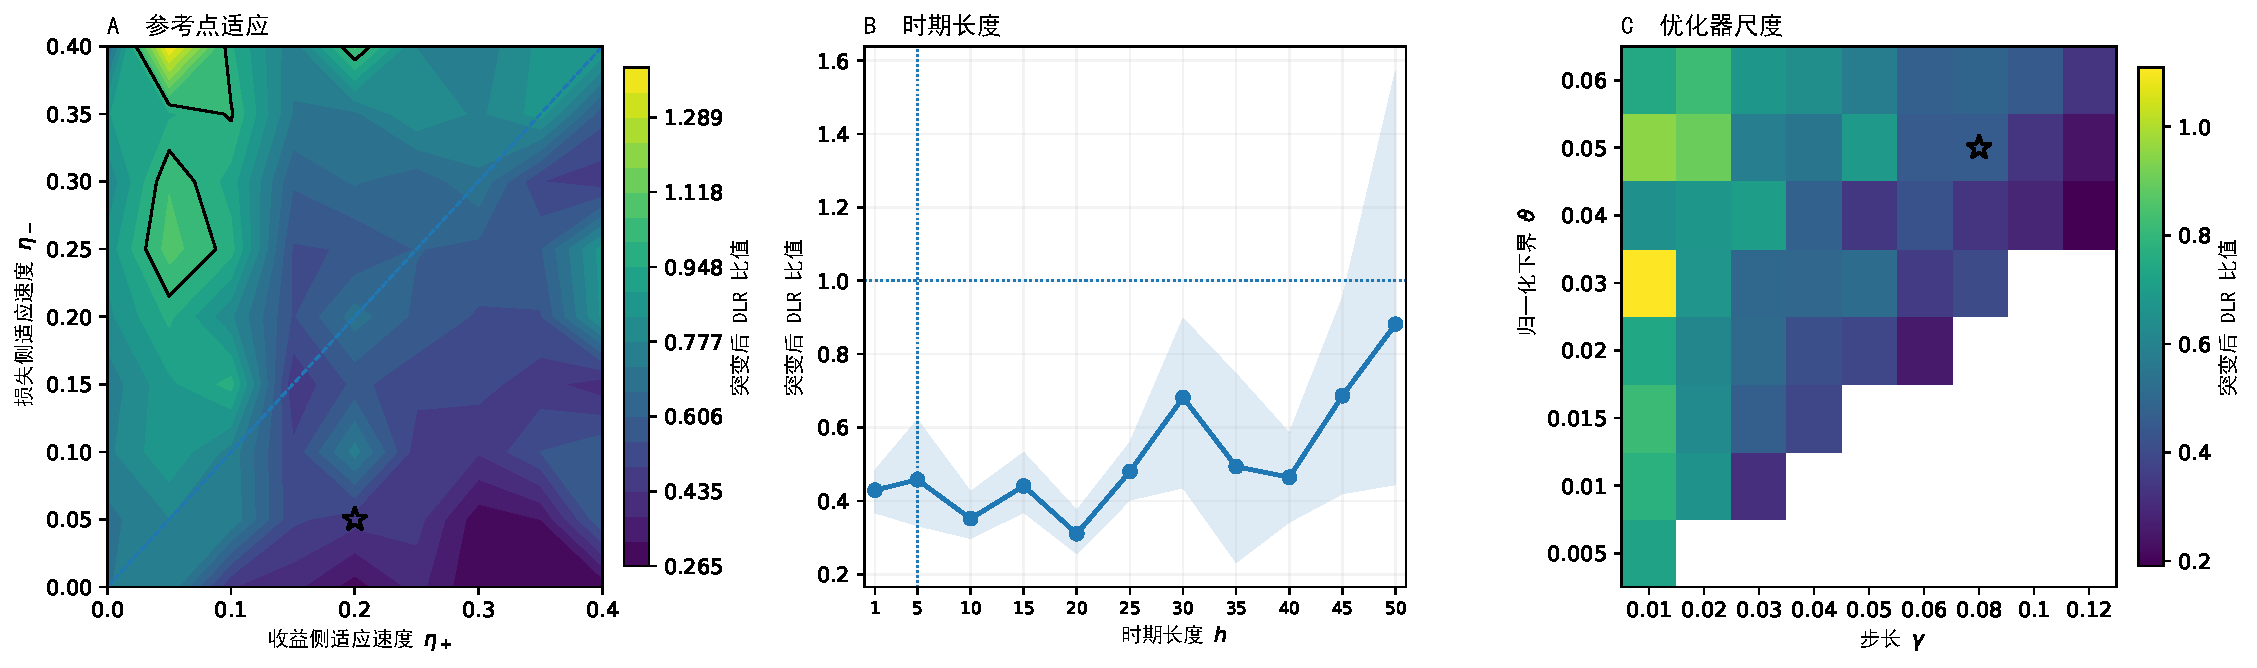
\includegraphics[width=\textwidth]{figures/e4_robustness_zh.pdf}
    \caption{参考点机制消融及在线跟踪优势的稳健性}
    \label{fig:e4-robustness}
\end{figure}

即使参考点完全不适应，$(\eta_+,\eta_-)=(0,0)$时的比值仍为$0.716$；八组正的对称适应配置也全部低于一，平均为$0.715$，其中六组的配对$95\%$区间完全低于一（图~\ref{fig:e4-robustness}A）。可见，持续更新本身已经能够改善移动市场中的一阶跟踪，非对称适应改变的是改善的幅度。

收益后的适应较快时，这一幅度更大。$36$组$\eta_+>\eta_-$配置的平均比值为$0.511$，全部点估计低于一，$33$组区间完全低于一。相反，$\eta_+<\eta_-$区域的平均比值为$0.826$；在$(\eta_+,\eta_-)=(0.05,0.40)$时，比值升至$1.403$，区间为$[1.224,1.552]$。同一市场路径中，参考点向收益适应更快会放大在线更新的优势，方向倒置且损失后适应很快时，这种优势甚至可能消失。

时期长度改变后，全部$11$个长度的平均比值仍低于一，其中$10$个配对区间完全低于一，只有$h=50$的区间跨过一（图~\ref{fig:e4-robustness}B）。在筛出的$48$组$(\gamma,\vartheta)$中，$47$组点估计低于一、$45$组区间完全低于一；唯一高于一的点估计对应区间为$[0.876,1.342]$（图~\ref{fig:e4-robustness}C）。因而，E3中看到的跟踪差距并不只出现在一个时期长度或一组更新参数上；对差距大小影响更明显的是参考点在收益与损失后的适应方向。

\FloatBarrier
\section{E5：真实市场投资组合评价}\label{sec:e5}

半合成市场能够指定何时突变，也能控制因子与收益的关系；真实市场不会按预设的规律切换。转入A股回放后，比较的重点因此从一阶残差变为实际价格路径上的收益、风险与调仓代价。资产池在测试期之前固定为沪深300的$300$只成分股，历史输入从2023年1月3日开始，样本外执行期为2025年1月2日至2026年5月29日。动量、反转、波动、估值、流动性、规模与前期持仓仅使用执行日前可获得的信息；质量因子要等财务数据公告后才进入策略。训练与实际账户执行均从同一个随机Dirichlet策略采样，每次调仓从财富中扣除$0.001\|\omega_t-\omega_{t-1}\|_1$的交易成本。

比较对象为DRCPT-PG、Symmetric CPT-PG、Static CPT-PG、Expected-Wealth PG与Exponential-Utility PG。五种方法共用五日时域、$\gamma=0.08$、预期轨迹预算$512$和预先设定的十个策略种子；DRCPT-PG的参考点参数为$(\eta_+,\eta_-)=(0.20,0.05)$。评价同时观察财富、年化收益与波动、Sharpe比率、最大回撤、换手和累计交易成本。

图~\ref{fig:e5-market}A展示十个种子的财富中位数及其离散带，B沿市场阶段观察回撤和恢复过程；C将期末财富与最大回撤对应，气泡面积反映换手；D比较平均换手和累计交易成本。这些视角分别衡量持有结果、下行风险与调仓代价。

\begin{figure}[!htbp]
    \centering
    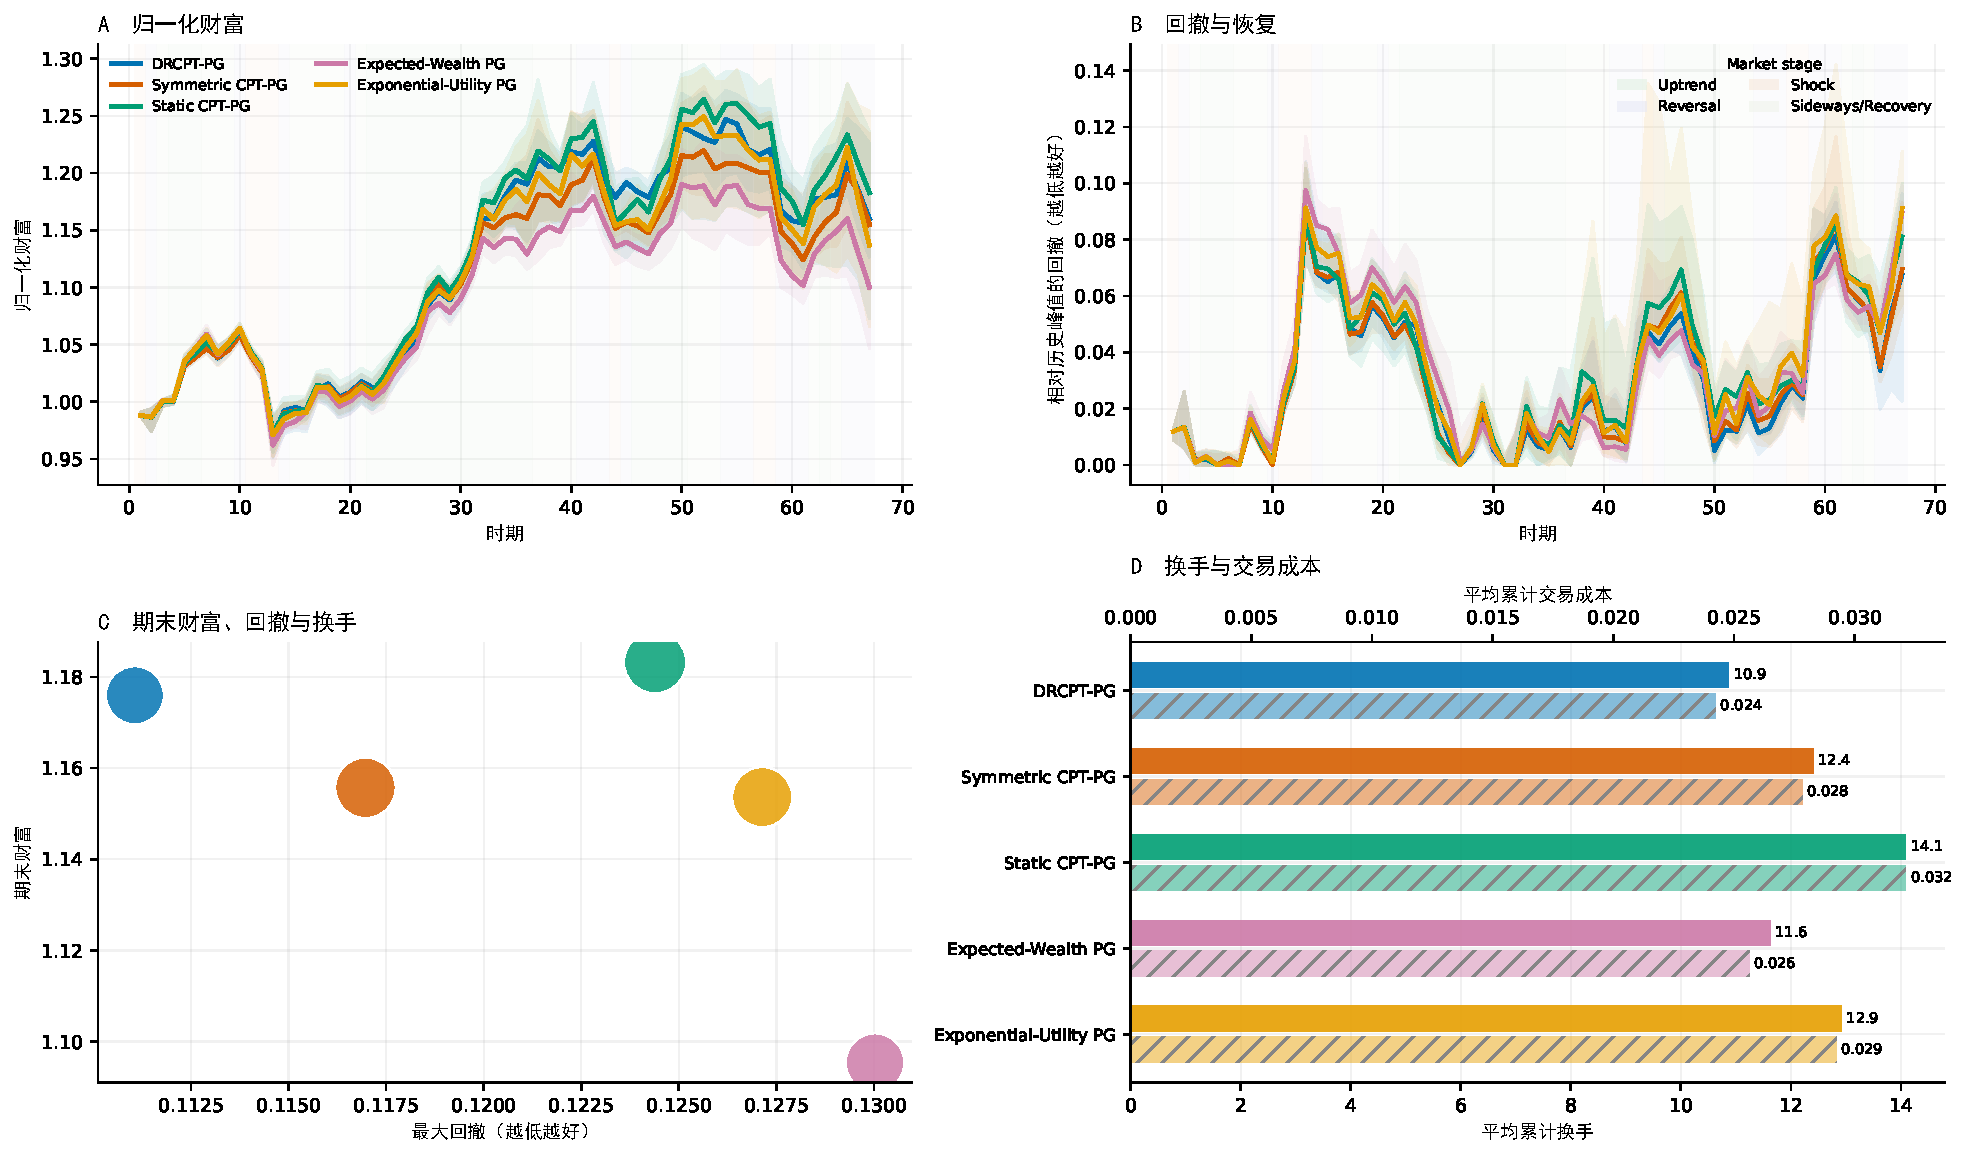
\includegraphics[width=\textwidth]{figures/figure_E5_external_validity_zh.pdf}
    \caption{A股时间顺序回放中的财富、回撤与交易成本}
    \label{fig:e5-market}
\end{figure}

\begin{table}[!htbp]
\centering
\footnotesize
\caption{E5真实市场结果，表中数值为十个策略种子的均值。}
\label{tab:e5-market}
\setlength{\tabcolsep}{3.5pt}
\begin{tabular}{lrrrrrr}
\toprule
方法 & 年化收益（\%） & 年化波动（\%） & Sharpe & 最大回撤（\%） & 总换手 & 交易成本（\%） \\
\midrule
DRCPT-PG & 13.03 & 15.62 & 0.856 & 11.67 & 10.87 & 2.42 \\
Symmetric CPT-PG & 13.21 & 16.35 & 0.796 & 12.48 & 12.41 & 2.78 \\
Static CPT-PG & 14.69 & 17.74 & 0.789 & 14.36 & 14.09 & 3.21 \\
Expected-Wealth PG & 10.51 & 16.68 & 0.606 & 14.23 & 11.63 & 2.56 \\
Exponential-Utility PG & 14.79 & 17.42 & 0.773 & 13.95 & 12.92 & 2.92 \\
\bottomrule
\end{tabular}
\end{table}

真实回放没有显示DRCPT-PG在平均收益上领先：它与直接的机制对照Symmetric CPT-PG的年化收益分别为$13.03\%$和$13.21\%$。差别主要在取得这份收益的过程。DRCPT-PG的平均Sharpe比率为$0.856$，在五种方法中最高；最大回撤为$11.67\%$，总换手与交易成本也最低（表~\ref{tab:e5-market}）。相较对称参考点，它以较低的波动、回撤和调仓代价获得了接近的收益。图~\ref{fig:e5-market}中的回撤路径和换手比较与这一结果一致：参考点机制在真实市场上更多改变了风险暴露与交易强度，而不是显著拉开期末财富。

\FloatBarrier
\section{E6：投资者行为预测}\label{sec:e6}

一个投资组合策略是否按动态参考点学习，与真实投资者是否也以变化的参考点判断持股，是两个不同的问题。为考察后者，取$306{,}444$次真实持股调仓机会，其中时间顺序测试集包含$71{,}854$次，以投资者下次调仓是否降低该股目标权重为因变量。四个logistic模型面对同一批决策，使用同样的标签、控制变量和时间划分；它们依次不使用参考点，或采用静态买入成本、对称动态、非对称动态参考点。最后一种取$(\eta_+,\eta_-)=(0.40,0.10)$。模型共同控制持有时间、前期权重、价格、投资者既往减持倾向，以及滞后的市场、组合和社交媒体汇总信息。配对不确定性由$200$次按投资者聚类的bootstrap估计。

对同一批真实决策，盈利与亏损状态分别按各模型的参考点划分。除样本外预测误差外，还观察股票价格高于自身参考点时的实际减持率、低于参考点时的减持率及两者之差。这使“能否预测减持”与“怎样识别盈利易卖、亏损易持”成为两个分别可以比较的问题。

图~\ref{fig:e6-behavior}A报告三种参考点相对无参考点模型在log loss和Brier score上的样本外改善；B给出各自盈亏划分下观察到的减持率，C比较两种状态的减持率之差，D再按投资者测试期以前的交易历史检查预测改善。A至C的区间均来自按投资者聚类的配对bootstrap。

\begin{figure}[!htbp]
    \centering
    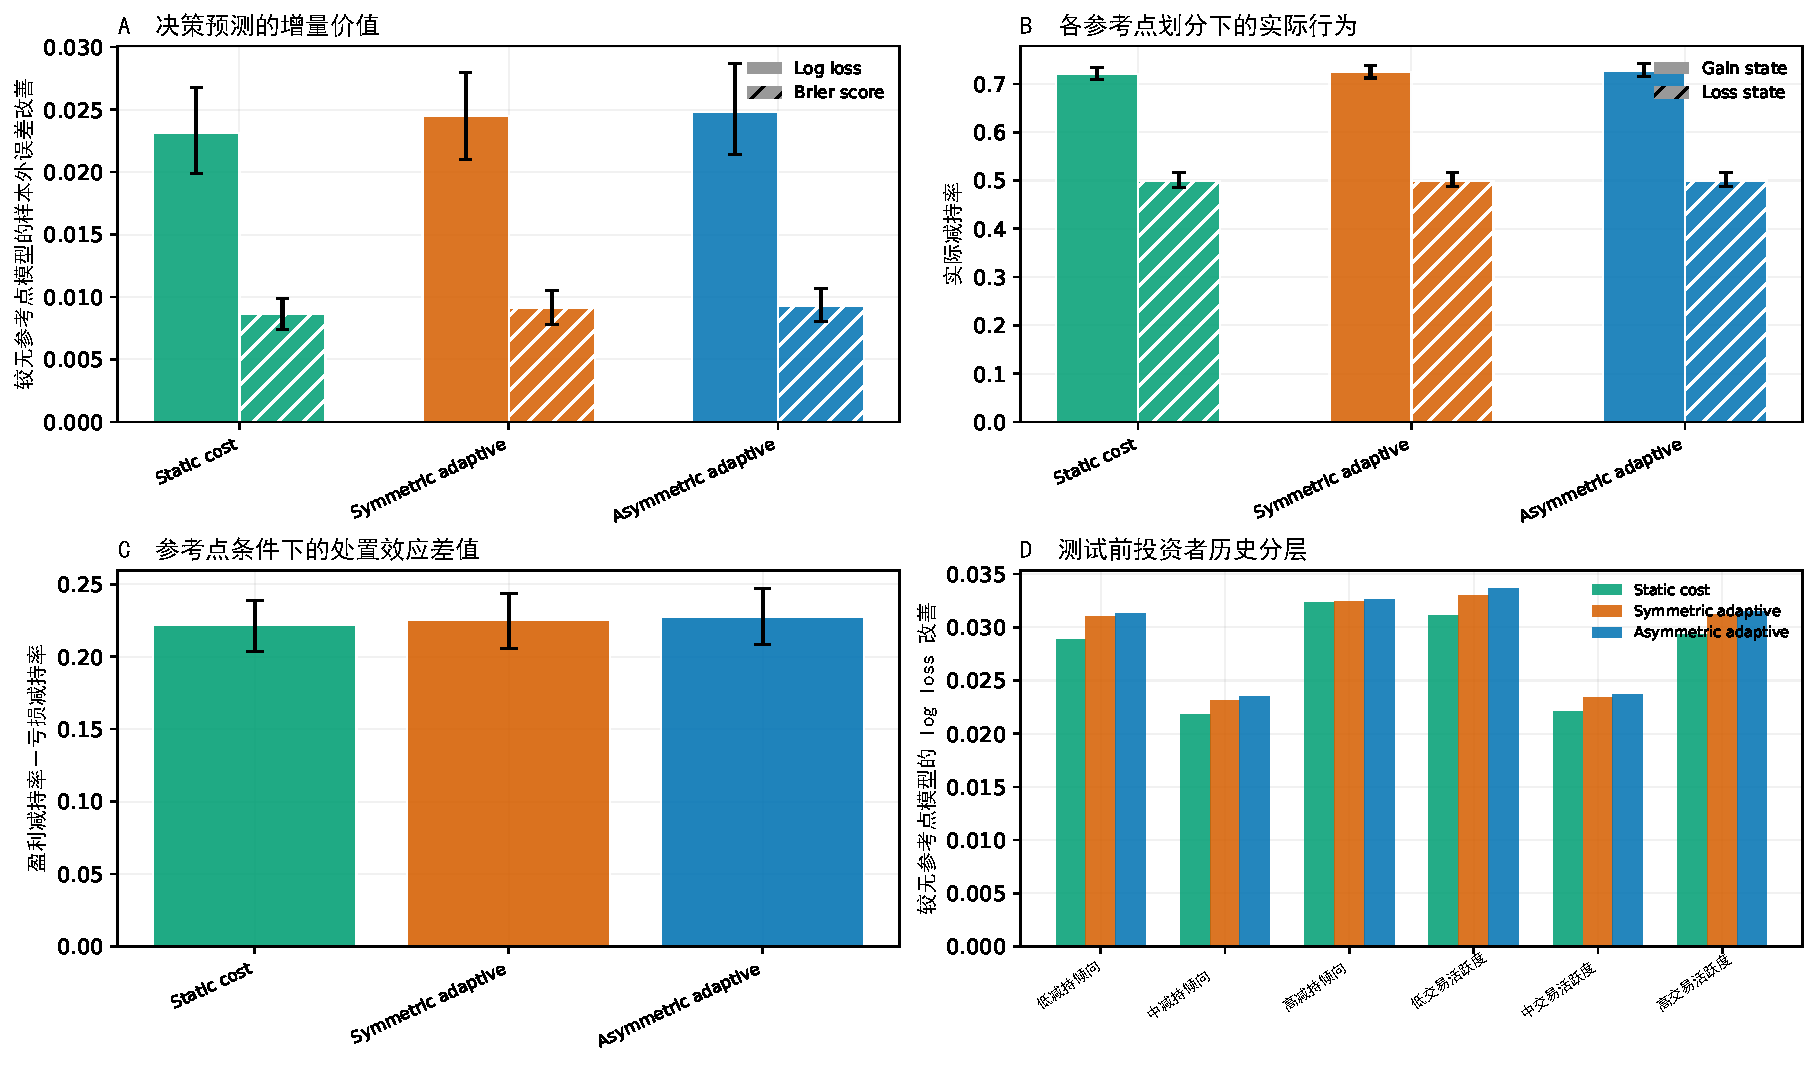
\includegraphics[width=\textwidth]{figures/figure_E6_behavior_alignment_zh.pdf}
    \caption{参考点与投资者减持行为的样本外比较}
    \label{fig:e6-behavior}
\end{figure}

在$71{,}854$次样本外决策上，模型能否知道股票相对于投资者参考点处于盈利还是亏损，比参考点如何适应更能影响预测。无参考点模型的log loss为$0.60420$，加入静态买入成本参考点后降至$0.58109$；对称动态和非对称动态参考点分别进一步降至$0.57975$与$0.57937$（图~\ref{fig:e6-behavior}A）。非对称模型相对无参考点模型的配对差值为$-0.02488$，$95\%$ bootstrap区间为$[-0.02866,-0.02142]$，其他预测指标也沿同一方向变化。

在已经考虑盈亏状态之后，参考点的更新方式仍有增量作用，但幅度小得多。非对称动态参考点相对静态参考点的log loss低$0.00174$，相对对称动态参考点低$0.000391$；后一个差值的配对区间为$[-0.000695,-0.000014]$。因此，样本外证据首先支持参考依赖的盈亏划分，其次才支持收益和损失后采用不同适应速度带来的额外预测信息。

预测误差之外，实际减持率也呈现一致的行为图景：不论采用哪种参考点，处于盈利状态的股票都比亏损股票更容易被减持。盈利与亏损减持率之差在静态、对称动态和非对称动态划分下依次为$0.2214$、$0.2250$和$0.2274$；非对称划分相对对称划分多$0.00255$，配对区间为$[0.00107,0.00404]$（图~\ref{fig:e6-behavior}B、C）。按投资者先前的交易历史分成六组后，非对称模型在每组的log loss改善也最大（图~\ref{fig:e6-behavior}D）。参考点适应的贡献虽小，但在预测减持与识别处置效应两个角度上方向一致。

\FloatBarrier
\section{E7：异质投资者模拟交互}\label{sec:e7}

真实持股决策表明，不同参考点对一次减持行为的解释力不同。若投资者反复收到组合建议，接受建议之后的评价又会怎样变化？这里沿用真实市场回放生成的建议，依据$3{,}481$名真实用户训练期的盈亏减持、交易活跃度、持仓分散程度、情绪及社交网络汇总信息，形成四类模拟投资者。中等交易频率且持仓集中的投资者占$49.4\%$，具有处置效应的投资者占$28.7\%$，活跃且分散投资者占$19.4\%$，低频且分散投资者占$2.5\%$。每类选取$16$名用户校准模拟规则，共有$64$名模拟投资者；分类只依据训练期行为，不以E6行为预测模型的全局系数决定类型。

五种策略梯度方法均提供现金加$300$只股票的组合建议。每个五日时期开始时，模拟投资者依据当前建议、由历史行为校准的偏好、建议与自身特征的匹配程度，以及此前的模型评价，决定是否采纳；这一决定发生在当期收益公布之前。采纳后执行建议五日，拒绝后维持原组合，两种路径都扣除交易成本并独立更新参考点。采纳后的条件满意度取该五日归一化前景价值与“不调仓”反事实之间的模型评价差；交互价值是采纳指示乘以这一差值，拒绝时为零。方法间使用配对的市场路径与采纳随机数，并按真实类型占比加权汇总。

图~\ref{fig:e7-agents}A给出四类模拟投资者的标准化行为特征，B和C分别比较不同类型对各方法的采纳率与采纳后的五日模型评价。D把各方法的采纳率和模型评价放在同一平面，气泡面积表示平均推荐匹配程度。这里的“满意度”始终是相对维持原持仓的模型前景价值差，不代表投资者报告的主观感受。

\begin{figure}[!htbp]
    \centering
    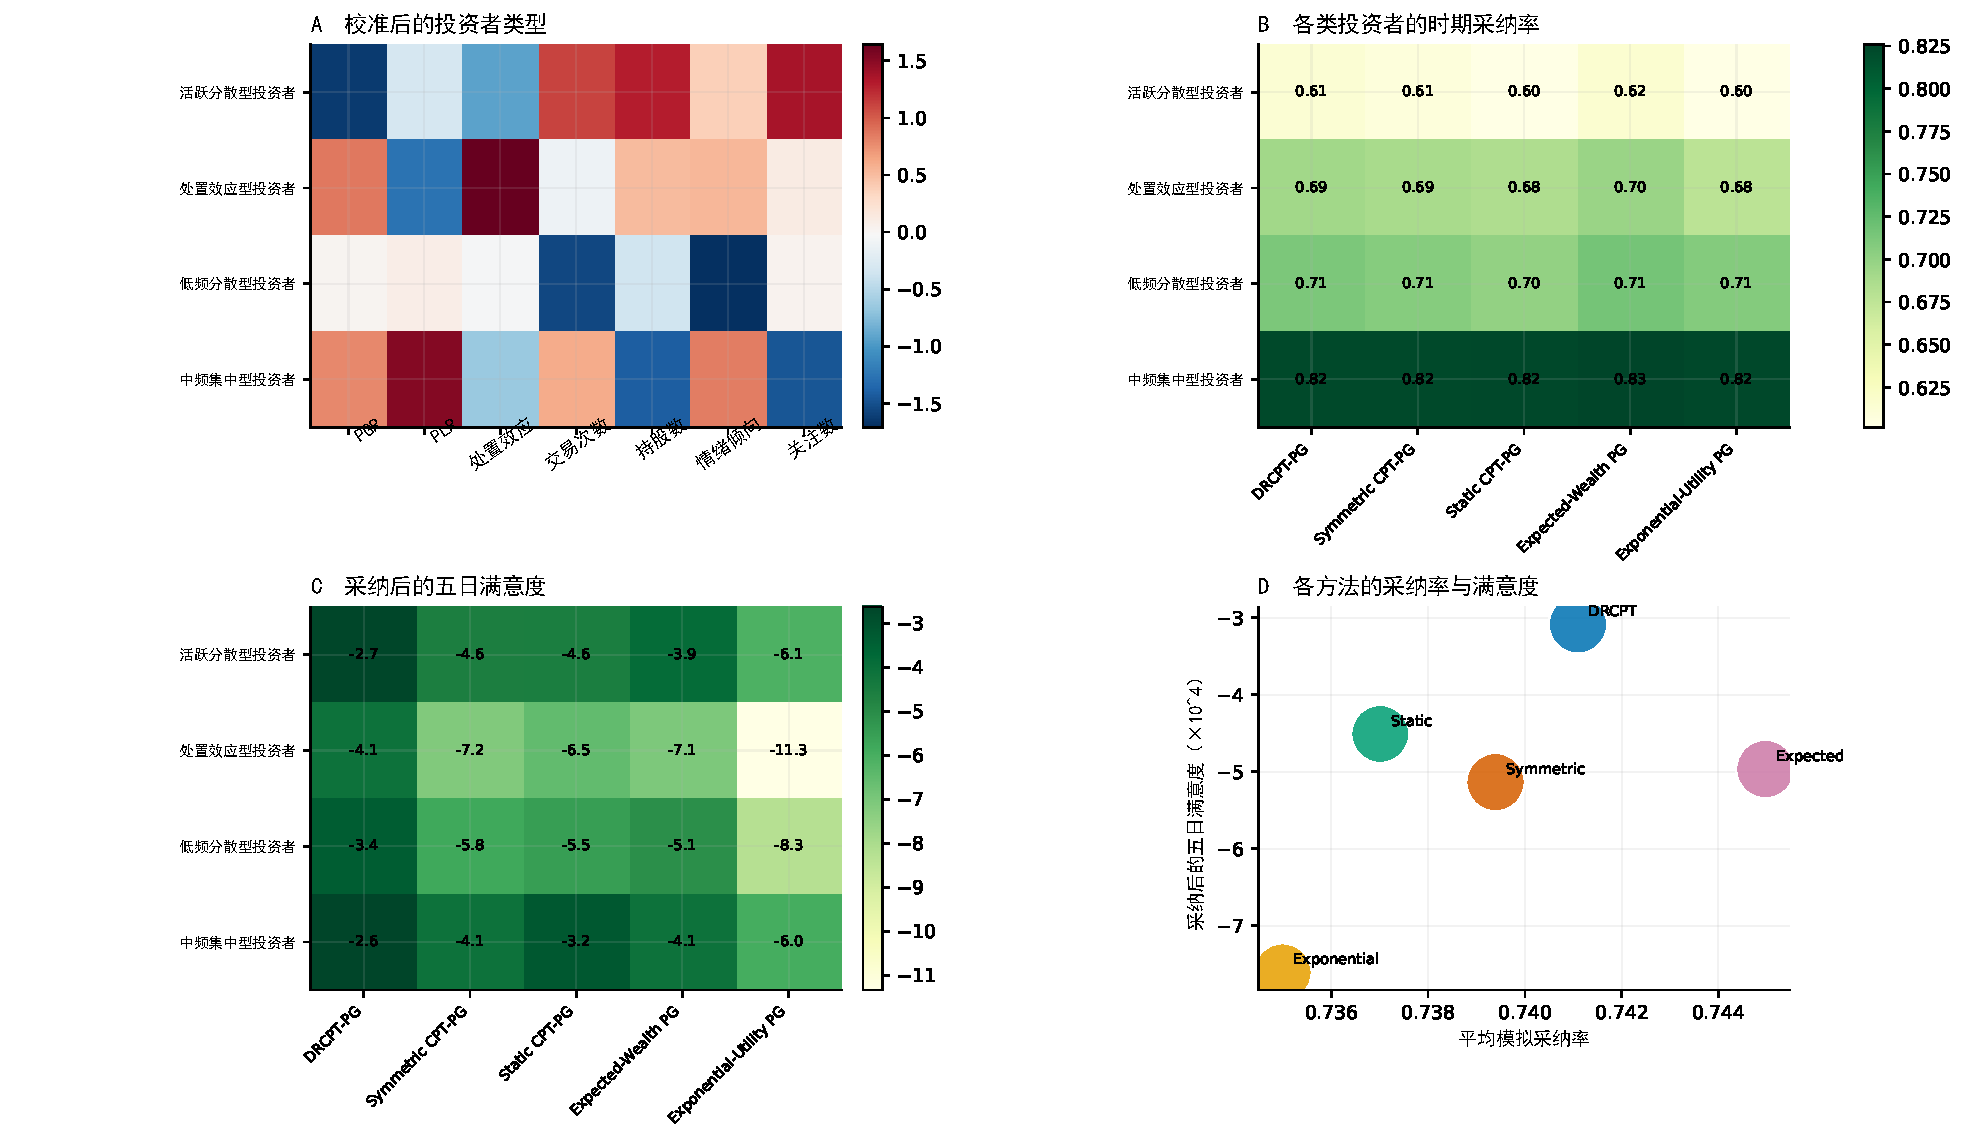
\includegraphics[width=\textwidth]{figures/figure_E7_heterogeneous_agents_zh.pdf}
    \caption{异质投资者的持续模拟交互}
    \label{fig:e7-agents}
\end{figure}

五种方法的加权模拟采纳率都接近四分之三，落在$0.735$至$0.745$之间；单看采纳意愿，难以判断建议执行后是否比维持原持仓更合适（图~\ref{fig:e7-agents}）。Expected-Wealth PG的采纳率略高，为$0.745$，采纳后的模型评价却低于DRCPT-PG。后者的采纳率为$0.741$，五日条件满意度为$-3.087\times10^{-4}$，采纳加权交互价值为$-2.265\times10^{-4}$，后二者在五种方法中最接近零。换言之，模拟投资者接受建议的频率相近，但DRCPT-PG执行后相对原持仓的负向前景评价较小；图~\ref{fig:e7-agents}D将这两个维度放在一起比较。

在活跃分散、处置效应、低频分散以及中等频率集中持仓的四类模拟投资者中，DRCPT-PG的采纳加权交互价值均为最高，其平均换手$9.29$和累计成本$0.0208$也是五种方法中最低的。五种方法相对“不调仓”的模型满意度均为负值；在这一共同评价尺度上，DRCPT-PG的负向差距最小。真实持股决策中的减持差异与模拟交互中的采纳后评价，分别从行为识别和连续推荐两个角度呈现了动态参考点的作用。
\FloatBarrier
\setcounter{secnumdepth}{4}
